\documentclass[1p]{elsarticle_modified}
%\bibliographystyle{elsarticle-num}

%\usepackage[colorlinks]{hyperref}
%\usepackage{abbrmath_seonhwa} %\Abb, \Ascr, \Acal ,\Abf, \Afrak
\usepackage{amsfonts}
\usepackage{amssymb}
\usepackage{amsmath}
\usepackage{amsthm}
\usepackage{scalefnt}
\usepackage{amsbsy}
\usepackage{kotex}
\usepackage{caption}
\usepackage{subfig}
\usepackage{color}
\usepackage{graphicx}
\usepackage{xcolor} %% white, black, red, green, blue, cyan, magenta, yellow
\usepackage{float}
\usepackage{setspace}
\usepackage{hyperref}

\usepackage{tikz}
\usetikzlibrary{arrows}

\usepackage{multirow}
\usepackage{array} % fixed length table
\usepackage{hhline}

%%%%%%%%%%%%%%%%%%%%%
\makeatletter
\renewcommand*\env@matrix[1][\arraystretch]{%
	\edef\arraystretch{#1}%
	\hskip -\arraycolsep
	\let\@ifnextchar\new@ifnextchar
	\array{*\c@MaxMatrixCols c}}
\makeatother %https://tex.stackexchange.com/questions/14071/how-can-i-increase-the-line-spacing-in-a-matrix
%%%%%%%%%%%%%%%

\usepackage[normalem]{ulem}

\newcommand{\msout}[1]{\ifmmode\text{\sout{\ensuremath{#1}}}\else\sout{#1}\fi}
%SOURCE: \msout is \stkout macro in https://tex.stackexchange.com/questions/20609/strikeout-in-math-mode

\newcommand{\cancel}[1]{
	\ifmmode
	{\color{red}\msout{#1}}
	\else
	{\color{red}\sout{#1}}
	\fi
}

\newcommand{\add}[1]{
	{\color{blue}\uwave{#1}}
}

\newcommand{\replace}[2]{
	\ifmmode
	{\color{red}\msout{#1}}{\color{blue}\uwave{#2}}
	\else
	{\color{red}\sout{#1}}{\color{blue}\uwave{#2}}
	\fi
}

\newcommand{\Sol}{\mathcal{S}} %segment
\newcommand{\D}{D} %diagram
\newcommand{\A}{\mathcal{A}} %arc


%%%%%%%%%%%%%%%%%%%%%%%%%%%%%5 test

\def\sl{\operatorname{\textup{SL}}(2,\Cbb)}
\def\psl{\operatorname{\textup{PSL}}(2,\Cbb)}
\def\quan{\mkern 1mu \triangleright \mkern 1mu}

\theoremstyle{definition}
\newtheorem{thm}{Theorem}[section]
\newtheorem{prop}[thm]{Proposition}
\newtheorem{lem}[thm]{Lemma}
\newtheorem{ques}[thm]{Question}
\newtheorem{cor}[thm]{Corollary}
\newtheorem{defn}[thm]{Definition}
\newtheorem{exam}[thm]{Example}
\newtheorem{rmk}[thm]{Remark}
\newtheorem{alg}[thm]{Algorithm}

\newcommand{\I}{\sqrt{-1}}
\begin{document}

%\begin{frontmatter}
%
%\title{Boundary parabolic representations of knots up to 8 crossings}
%
%%% Group authors per affiliation:
%\author{Yunhi Cho} 
%\address{Department of Mathematics, University of Seoul, Seoul, Korea}
%\ead{yhcho@uos.ac.kr}
%
%
%\author{Seonhwa Kim} %\fnref{s_kim}}
%\address{Center for Geometry and Physics, Institute for Basic Science, Pohang, 37673, Korea}
%\ead{ryeona17@ibs.re.kr}
%
%\author{Hyuk Kim}
%\address{Department of Mathematical Sciences, Seoul National University, Seoul 08826, Korea}
%\ead{hyukkim@snu.ac.kr}
%
%\author{Seokbeom Yoon}
%\address{Department of Mathematical Sciences, Seoul National University, Seoul, 08826,  Korea}
%\ead{sbyoon15@snu.ac.kr}
%
%\begin{abstract}
%We find all boundary parabolic representation of knots up to 8 crossings.
%
%\end{abstract}
%\begin{keyword}
%    \MSC[2010] 57M25 
%\end{keyword}
%
%\end{frontmatter}

%\linenumbers
%\tableofcontents
%
\newcommand\colored[1]{\textcolor{white}{\rule[-0.35ex]{0.8em}{1.4ex}}\kern-0.8em\color{red} #1}%
%\newcommand\colored[1]{\textcolor{white}{ #1}\kern-2.17ex	\textcolor{white}{ #1}\kern-1.81ex	\textcolor{white}{ #1}\kern-2.15ex\color{red}#1	}

{\Large $\underline{12a_{0685}~(K12a_{0685})}$}

\setlength{\tabcolsep}{10pt}
\renewcommand{\arraystretch}{1.6}
\vspace{1cm}\begin{tabular}{m{100pt}>{\centering\arraybackslash}m{274pt}}
\multirow{5}{120pt}{
	\centering
	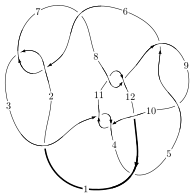
\includegraphics[width=112pt]{../../../GIT/diagram.site/Diagrams/png/1486_12a_0685.png}\\
\ \ \ A knot diagram\footnotemark}&
\allowdisplaybreaks
\textbf{Linearized knot diagam} \\
\cline{2-2}
 &
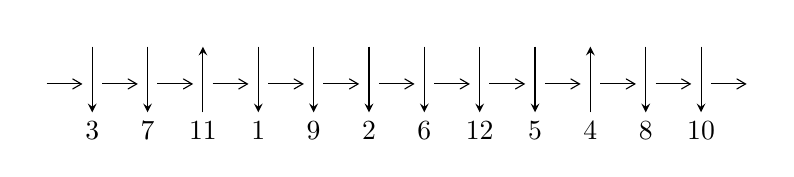
\begin{tikzpicture}[x=20pt, y=17pt]
	% nodes
	\node (C0) at (0, 0) {};
	\node (C1) at (1, 0) {};
	\node (C1U) at (1, +1) {};
	\node (C1D) at (1, -1) {3};

	\node (C2) at (2, 0) {};
	\node (C2U) at (2, +1) {};
	\node (C2D) at (2, -1) {7};

	\node (C3) at (3, 0) {};
	\node (C3U) at (3, +1) {};
	\node (C3D) at (3, -1) {11};

	\node (C4) at (4, 0) {};
	\node (C4U) at (4, +1) {};
	\node (C4D) at (4, -1) {1};

	\node (C5) at (5, 0) {};
	\node (C5U) at (5, +1) {};
	\node (C5D) at (5, -1) {9};

	\node (C6) at (6, 0) {};
	\node (C6U) at (6, +1) {};
	\node (C6D) at (6, -1) {2};

	\node (C7) at (7, 0) {};
	\node (C7U) at (7, +1) {};
	\node (C7D) at (7, -1) {6};

	\node (C8) at (8, 0) {};
	\node (C8U) at (8, +1) {};
	\node (C8D) at (8, -1) {12};

	\node (C9) at (9, 0) {};
	\node (C9U) at (9, +1) {};
	\node (C9D) at (9, -1) {5};

	\node (C10) at (10, 0) {};
	\node (C10U) at (10, +1) {};
	\node (C10D) at (10, -1) {4};

	\node (C11) at (11, 0) {};
	\node (C11U) at (11, +1) {};
	\node (C11D) at (11, -1) {8};

	\node (C12) at (12, 0) {};
	\node (C12U) at (12, +1) {};
	\node (C12D) at (12, -1) {10};
	\node (C13) at (13, 0) {};

	% arrows
	\draw[->,>={angle 60}]
	(C0) edge (C1) (C1) edge (C2) (C2) edge (C3) (C3) edge (C4) (C4) edge (C5) (C5) edge (C6) (C6) edge (C7) (C7) edge (C8) (C8) edge (C9) (C9) edge (C10) (C10) edge (C11) (C11) edge (C12) (C12) edge (C13) ;	\draw[->,>=stealth]
	(C1U) edge (C1D) (C2U) edge (C2D) (C3D) edge (C3U) (C4U) edge (C4D) (C5U) edge (C5D) (C6U) edge (C6D) (C7U) edge (C7D) (C8U) edge (C8D) (C9U) edge (C9D) (C10D) edge (C10U) (C11U) edge (C11D) (C12U) edge (C12D) ;
	\end{tikzpicture} \\
\hhline{~~} \\& 
\textbf{Solving Sequence} \\ \cline{2-2} 
 &
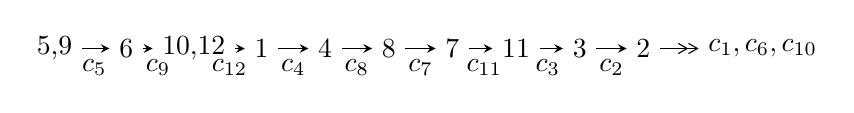
\begin{tikzpicture}[x=23pt, y=7pt]
	% node
	\node (A0) at (-1/8, 0) {5,9};
	\node (A1) at (1, 0) {6};
	\node (A2) at (33/16, 0) {10,12};
	\node (A3) at (25/8, 0) {1};
	\node (A4) at (33/8, 0) {4};
	\node (A5) at (41/8, 0) {8};
	\node (A6) at (49/8, 0) {7};
	\node (A7) at (57/8, 0) {11};
	\node (A8) at (65/8, 0) {3};
	\node (A9) at (73/8, 0) {2};
	\node (C1) at (1/2, -1) {$c_{5}$};
	\node (C2) at (3/2, -1) {$c_{9}$};
	\node (C3) at (21/8, -1) {$c_{12}$};
	\node (C4) at (29/8, -1) {$c_{4}$};
	\node (C5) at (37/8, -1) {$c_{8}$};
	\node (C6) at (45/8, -1) {$c_{7}$};
	\node (C7) at (53/8, -1) {$c_{11}$};
	\node (C8) at (61/8, -1) {$c_{3}$};
	\node (C9) at (69/8, -1) {$c_{2}$};
	\node (A10) at (11, 0) {$c_{1},c_{6},c_{10}$};

	% edge
	\draw[->,>=stealth]	
	(A0) edge (A1) (A1) edge (A2) (A2) edge (A3) (A3) edge (A4) (A4) edge (A5) (A5) edge (A6) (A6) edge (A7) (A7) edge (A8) (A8) edge (A9) ;
	\draw[->>,>={angle 60}]	
	(A9) edge (A10);
\end{tikzpicture} \\ 

\end{tabular} \\

\footnotetext{
The image of knot diagram is generated by the software ``\textbf{Draw programme}" developed by Andrew Bartholomew(\url{http://www.layer8.co.uk/maths/draw/index.htm\#Running-draw}), where we modified some parts for our purpose(\url{https://github.com/CATsTAILs/LinksPainter}).
}\phantom \\ \newline 
\centering \textbf{Ideals for irreducible components\footnotemark of $X_{\text{par}}$} 
 
\begin{align*}
I^u_{1}&=\langle 
-2.88356\times10^{553} u^{121}+1.21209\times10^{554} u^{120}+\cdots+8.71696\times10^{553} b-3.64779\times10^{555},\\
\phantom{I^u_{1}}&\phantom{= \langle  }4.27797\times10^{555} u^{121}-1.73052\times10^{556} u^{120}+\cdots+2.72841\times10^{556} a+1.06739\times10^{558},\\
\phantom{I^u_{1}}&\phantom{= \langle  }u^{122}-5 u^{121}+\cdots-2671 u+313\rangle \\
I^u_{2}&=\langle 
5 u^{19}-5 u^{18}+\cdots+b-13 u,\;-4 u^{19}+4 u^{18}+\cdots+a+13 u,\;u^{20}- u^{19}+\cdots-4 u^2-1\rangle \\
I^u_{3}&=\langle 
b+1,\;a- u-1,\;u^2+u+1\rangle \\
\\
\end{align*}
\raggedright * 3 irreducible components of $\dim_{\mathbb{C}}=0$, with total 144 representations.\\
\footnotetext{All coefficients of polynomials are rational numbers. But the coefficients are sometimes approximated in decimal forms when there is not enough margin.}
\newpage
\renewcommand{\arraystretch}{1}
\centering \section*{I. $I^u_{1}= \langle -2.88\times10^{553} u^{121}+1.21\times10^{554} u^{120}+\cdots+8.72\times10^{553} b-3.65\times10^{555},\;4.28\times10^{555} u^{121}-1.73\times10^{556} u^{120}+\cdots+2.73\times10^{556} a+1.07\times10^{558},\;u^{122}-5 u^{121}+\cdots-2671 u+313 \rangle$}
\flushleft \textbf{(i) Arc colorings}\\
\begin{tabular}{m{7pt} m{180pt} m{7pt} m{180pt} }
\flushright $a_{5}=$&$\begin{pmatrix}1\\0\end{pmatrix}$ \\
\flushright $a_{9}=$&$\begin{pmatrix}0\\u\end{pmatrix}$ \\
\flushright $a_{6}=$&$\begin{pmatrix}1\\u^2\end{pmatrix}$ \\
\flushright $a_{10}=$&$\begin{pmatrix}- u\\u\end{pmatrix}$ \\
\flushright $a_{12}=$&$\begin{pmatrix}-0.156793 u^{121}+0.634260 u^{120}+\cdots+256.687 u-39.1212\\0.330799 u^{121}-1.39049 u^{120}+\cdots-256.314 u+41.8470\end{pmatrix}$ \\
\flushright $a_{1}=$&$\begin{pmatrix}-0.0146363 u^{121}+0.105168 u^{120}+\cdots+7.19887 u-3.50278\\0.188642 u^{121}-0.861399 u^{120}+\cdots-6.82568 u+6.22859\end{pmatrix}$ \\
\flushright $a_{4}=$&$\begin{pmatrix}0.560056 u^{121}-2.92442 u^{120}+\cdots+643.200 u-60.0524\\-0.342976 u^{121}+1.55630 u^{120}+\cdots+93.8076 u-22.7278\end{pmatrix}$ \\
\flushright $a_{8}=$&$\begin{pmatrix}0.101891 u^{121}-0.649364 u^{120}+\cdots+517.201 u-55.0592\\-0.436544 u^{121}+2.01244 u^{120}+\cdots-9.53506 u-14.2558\end{pmatrix}$ \\
\flushright $a_{7}=$&$\begin{pmatrix}-0.229119 u^{121}+0.737054 u^{120}+\cdots+913.255 u-113.107\\-0.130498 u^{121}+0.841269 u^{120}+\cdots-623.444 u+69.8259\end{pmatrix}$ \\
\flushright $a_{11}=$&$\begin{pmatrix}0.423648 u^{121}-1.77534 u^{120}+\cdots-508.989 u+67.2783\\-0.822229 u^{121}+3.70501 u^{120}+\cdots+315.069 u-65.2216\end{pmatrix}$ \\
\flushright $a_{3}=$&$\begin{pmatrix}-0.149715 u^{121}+0.0244993 u^{120}+\cdots+1701.15 u-213.253\\0.0916345 u^{121}+0.419588 u^{120}+\cdots-2068.61 u+254.915\end{pmatrix}$ \\
\flushright $a_{2}=$&$\begin{pmatrix}-0.0978973 u^{121}+0.243033 u^{120}+\cdots+277.019 u-36.7654\\-0.183988 u^{121}+1.22389 u^{120}+\cdots-801.640 u+90.3639\end{pmatrix}$\\&\end{tabular}
\flushleft \textbf{(ii) Obstruction class $= -1$}\\~\\
\flushleft \textbf{(iii) Cusp Shapes $= 0.345389 u^{121}-0.408893 u^{120}+\cdots-2814.41 u+346.625$}\\~\\
\newpage\renewcommand{\arraystretch}{1}
\flushleft \textbf{(iv) u-Polynomials at the component}\newline \\
\begin{tabular}{m{50pt}|m{274pt}}
Crossings & \hspace{64pt}u-Polynomials at each crossing \\
\hline $$\begin{aligned}c_{1},c_{7}\end{aligned}$$&$\begin{aligned}
&u^{122}+41 u^{121}+\cdots+33207 u+121
\end{aligned}$\\
\hline $$\begin{aligned}c_{2},c_{6}\end{aligned}$$&$\begin{aligned}
&u^{122}- u^{121}+\cdots+223 u+11
\end{aligned}$\\
\hline $$\begin{aligned}c_{3},c_{10}\end{aligned}$$&$\begin{aligned}
&u^{122}-2 u^{121}+\cdots+169938 u+8767
\end{aligned}$\\
\hline $$\begin{aligned}c_{4}\end{aligned}$$&$\begin{aligned}
&u^{122}-6 u^{121}+\cdots+12 u-8
\end{aligned}$\\
\hline $$\begin{aligned}c_{5},c_{9}\end{aligned}$$&$\begin{aligned}
&u^{122}-5 u^{121}+\cdots-2671 u+313
\end{aligned}$\\
\hline $$\begin{aligned}c_{8},c_{11}\end{aligned}$$&$\begin{aligned}
&u^{122}+u^{121}+\cdots+4149 u+108
\end{aligned}$\\
\hline $$\begin{aligned}c_{12}\end{aligned}$$&$\begin{aligned}
&u^{122}-2 u^{121}+\cdots+29 u-1
\end{aligned}$\\
\hline
\end{tabular}\\~\\
\newpage\renewcommand{\arraystretch}{1}
\flushleft \textbf{(v) Riley Polynomials at the component}\newline \\
\begin{tabular}{m{50pt}|m{274pt}}
Crossings & \hspace{64pt}Riley Polynomials at each crossing \\
\hline $$\begin{aligned}c_{1},c_{7}\end{aligned}$$&$\begin{aligned}
&y^{122}+91 y^{121}+\cdots-1012244039 y+14641
\end{aligned}$\\
\hline $$\begin{aligned}c_{2},c_{6}\end{aligned}$$&$\begin{aligned}
&y^{122}-41 y^{121}+\cdots-33207 y+121
\end{aligned}$\\
\hline $$\begin{aligned}c_{3},c_{10}\end{aligned}$$&$\begin{aligned}
&y^{122}+70 y^{121}+\cdots+180016550 y+76860289
\end{aligned}$\\
\hline $$\begin{aligned}c_{4}\end{aligned}$$&$\begin{aligned}
&y^{122}+20 y^{121}+\cdots+720 y+64
\end{aligned}$\\
\hline $$\begin{aligned}c_{5},c_{9}\end{aligned}$$&$\begin{aligned}
&y^{122}+73 y^{121}+\cdots+3716843 y+97969
\end{aligned}$\\
\hline $$\begin{aligned}c_{8},c_{11}\end{aligned}$$&$\begin{aligned}
&y^{122}-73 y^{121}+\cdots-13689081 y+11664
\end{aligned}$\\
\hline $$\begin{aligned}c_{12}\end{aligned}$$&$\begin{aligned}
&y^{122}-12 y^{121}+\cdots-81 y+1
\end{aligned}$\\
\hline
\end{tabular}\\~\\
\newpage\flushleft \textbf{(vi) Complex Volumes and Cusp Shapes}
$$\begin{array}{c|c|c}  
\text{Solutions to }I^u_{1}& \I (\text{vol} + \sqrt{-1}CS) & \text{Cusp shape}\\
 \hline 
\begin{aligned}
u &= -0.507146 + 0.855992 I \\
a &= \phantom{-}1.39763 + 0.38908 I \\
b &= -1.58922 - 0.73202 I\end{aligned}
 & \phantom{-}0.15714 + 3.46101 I & \phantom{-0.000000 } 0 \\ \hline\begin{aligned}
u &= -0.507146 - 0.855992 I \\
a &= \phantom{-}1.39763 - 0.38908 I \\
b &= -1.58922 + 0.73202 I\end{aligned}
 & \phantom{-}0.15714 - 3.46101 I & \phantom{-0.000000 } 0 \\ \hline\begin{aligned}
u &= \phantom{-}0.242227 + 0.979225 I \\
a &= \phantom{-}0.651388 - 0.786992 I \\
b &= -1.76441 + 0.84561 I\end{aligned}
 & -1.76184 - 1.89377 I & \phantom{-0.000000 } 0 \\ \hline\begin{aligned}
u &= \phantom{-}0.242227 - 0.979225 I \\
a &= \phantom{-}0.651388 + 0.786992 I \\
b &= -1.76441 - 0.84561 I\end{aligned}
 & -1.76184 + 1.89377 I & \phantom{-0.000000 } 0 \\ \hline\begin{aligned}
u &= \phantom{-}0.369913 + 0.912696 I \\
a &= -1.21901 + 0.99429 I \\
b &= \phantom{-}1.33892 - 1.30519 I\end{aligned}
 & -5.98273 - 3.58080 I & \phantom{-0.000000 } 0 \\ \hline\begin{aligned}
u &= \phantom{-}0.369913 - 0.912696 I \\
a &= -1.21901 - 0.99429 I \\
b &= \phantom{-}1.33892 + 1.30519 I\end{aligned}
 & -5.98273 + 3.58080 I & \phantom{-0.000000 } 0 \\ \hline\begin{aligned}
u &= -0.721993 + 0.658333 I \\
a &= -0.524412 - 1.175230 I \\
b &= -0.362442 + 0.593749 I\end{aligned}
 & -0.417036 + 1.284330 I & \phantom{-0.000000 } 0 \\ \hline\begin{aligned}
u &= -0.721993 - 0.658333 I \\
a &= -0.524412 + 1.175230 I \\
b &= -0.362442 - 0.593749 I\end{aligned}
 & -0.417036 - 1.284330 I & \phantom{-0.000000 } 0 \\ \hline\begin{aligned}
u &= \phantom{-}0.648403 + 0.720029 I \\
a &= \phantom{-}0.41433 - 1.40827 I \\
b &= \phantom{-}0.393075 + 0.699599 I\end{aligned}
 & -1.05367 + 4.67798 I & \phantom{-0.000000 } 0 \\ \hline\begin{aligned}
u &= \phantom{-}0.648403 - 0.720029 I \\
a &= \phantom{-}0.41433 + 1.40827 I \\
b &= \phantom{-}0.393075 - 0.699599 I\end{aligned}
 & -1.05367 - 4.67798 I & \phantom{-0.000000 } 0\\
 \hline 
 \end{array}$$\newpage$$\begin{array}{c|c|c}  
\text{Solutions to }I^u_{1}& \I (\text{vol} + \sqrt{-1}CS) & \text{Cusp shape}\\
 \hline 
\begin{aligned}
u &= \phantom{-}0.227753 + 1.007340 I \\
a &= \phantom{-}0.479723 + 0.520123 I \\
b &= -1.72903 + 0.21460 I\end{aligned}
 & \phantom{-}1.31833 - 3.84074 I & \phantom{-0.000000 } 0 \\ \hline\begin{aligned}
u &= \phantom{-}0.227753 - 1.007340 I \\
a &= \phantom{-}0.479723 - 0.520123 I \\
b &= -1.72903 - 0.21460 I\end{aligned}
 & \phantom{-}1.31833 + 3.84074 I & \phantom{-0.000000 } 0 \\ \hline\begin{aligned}
u &= -0.523794 + 0.893580 I \\
a &= \phantom{-}0.413860 + 0.269007 I \\
b &= -0.395349 + 0.457081 I\end{aligned}
 & -1.71998 + 0.88588 I & \phantom{-0.000000 } 0 \\ \hline\begin{aligned}
u &= -0.523794 - 0.893580 I \\
a &= \phantom{-}0.413860 - 0.269007 I \\
b &= -0.395349 - 0.457081 I\end{aligned}
 & -1.71998 - 0.88588 I & \phantom{-0.000000 } 0 \\ \hline\begin{aligned}
u &= \phantom{-}0.036474 + 0.957207 I \\
a &= \phantom{-}0.01900 - 2.30092 I \\
b &= \phantom{-}0.028206 + 1.126470 I\end{aligned}
 & -3.98184 - 2.64884 I & \phantom{-0.000000 } 0 \\ \hline\begin{aligned}
u &= \phantom{-}0.036474 - 0.957207 I \\
a &= \phantom{-}0.01900 + 2.30092 I \\
b &= \phantom{-}0.028206 - 1.126470 I\end{aligned}
 & -3.98184 + 2.64884 I & \phantom{-0.000000 } 0 \\ \hline\begin{aligned}
u &= \phantom{-}0.144312 + 1.033520 I \\
a &= -0.43604 + 1.42034 I \\
b &= \phantom{-}0.47698 - 1.68915 I\end{aligned}
 & -3.56343 + 2.07493 I & \phantom{-0.000000 } 0 \\ \hline\begin{aligned}
u &= \phantom{-}0.144312 - 1.033520 I \\
a &= -0.43604 - 1.42034 I \\
b &= \phantom{-}0.47698 + 1.68915 I\end{aligned}
 & -3.56343 - 2.07493 I & \phantom{-0.000000 } 0 \\ \hline\begin{aligned}
u &= \phantom{-}0.618887 + 0.841397 I \\
a &= \phantom{-}0.233538 - 0.401885 I \\
b &= -1.47477 + 0.40985 I\end{aligned}
 & \phantom{-}0.75469 - 3.02592 I & \phantom{-0.000000 } 0 \\ \hline\begin{aligned}
u &= \phantom{-}0.618887 - 0.841397 I \\
a &= \phantom{-}0.233538 + 0.401885 I \\
b &= -1.47477 - 0.40985 I\end{aligned}
 & \phantom{-}0.75469 + 3.02592 I & \phantom{-0.000000 } 0\\
 \hline 
 \end{array}$$\newpage$$\begin{array}{c|c|c}  
\text{Solutions to }I^u_{1}& \I (\text{vol} + \sqrt{-1}CS) & \text{Cusp shape}\\
 \hline 
\begin{aligned}
u &= \phantom{-}0.477079 + 0.822515 I \\
a &= -1.59165 + 0.48054 I \\
b &= \phantom{-}1.76249 - 0.84223 I\end{aligned}
 & -0.77649 - 9.14865 I & \phantom{-0.000000 } 0 \\ \hline\begin{aligned}
u &= \phantom{-}0.477079 - 0.822515 I \\
a &= -1.59165 - 0.48054 I \\
b &= \phantom{-}1.76249 + 0.84223 I\end{aligned}
 & -0.77649 + 9.14865 I & \phantom{-0.000000 } 0 \\ \hline\begin{aligned}
u &= \phantom{-}1.054680 + 0.094255 I \\
a &= \phantom{-}1.218420 - 0.371226 I \\
b &= -0.244011 - 0.244100 I\end{aligned}
 & -9.21798 + 6.22997 I & \phantom{-0.000000 } 0 \\ \hline\begin{aligned}
u &= \phantom{-}1.054680 - 0.094255 I \\
a &= \phantom{-}1.218420 + 0.371226 I \\
b &= -0.244011 + 0.244100 I\end{aligned}
 & -9.21798 - 6.22997 I & \phantom{-0.000000 } 0 \\ \hline\begin{aligned}
u &= \phantom{-}0.138610 + 1.058360 I \\
a &= -0.532185 + 1.199180 I \\
b &= \phantom{-}1.139570 + 0.187880 I\end{aligned}
 & \phantom{-}3.72323 - 4.84674 I & \phantom{-0.000000 } 0 \\ \hline\begin{aligned}
u &= \phantom{-}0.138610 - 1.058360 I \\
a &= -0.532185 - 1.199180 I \\
b &= \phantom{-}1.139570 - 0.187880 I\end{aligned}
 & \phantom{-}3.72323 + 4.84674 I & \phantom{-0.000000 } 0 \\ \hline\begin{aligned}
u &= -0.359693 + 1.007070 I \\
a &= \phantom{-}0.432069 - 0.378673 I \\
b &= -1.106490 + 0.143329 I\end{aligned}
 & \phantom{-}1.61424 + 3.30812 I & \phantom{-0.000000 } 0 \\ \hline\begin{aligned}
u &= -0.359693 - 1.007070 I \\
a &= \phantom{-}0.432069 + 0.378673 I \\
b &= -1.106490 - 0.143329 I\end{aligned}
 & \phantom{-}1.61424 - 3.30812 I & \phantom{-0.000000 } 0 \\ \hline\begin{aligned}
u &= -0.917118 + 0.113358 I \\
a &= -1.316600 - 0.058252 I \\
b &= \phantom{-}0.079637 + 0.366292 I\end{aligned}
 & -5.18540 + 3.19989 I & \phantom{-0.000000 } 0 \\ \hline\begin{aligned}
u &= -0.917118 - 0.113358 I \\
a &= -1.316600 + 0.058252 I \\
b &= \phantom{-}0.079637 - 0.366292 I\end{aligned}
 & -5.18540 - 3.19989 I & \phantom{-0.000000 } 0\\
 \hline 
 \end{array}$$\newpage$$\begin{array}{c|c|c}  
\text{Solutions to }I^u_{1}& \I (\text{vol} + \sqrt{-1}CS) & \text{Cusp shape}\\
 \hline 
\begin{aligned}
u &= -0.071921 + 1.074860 I \\
a &= \phantom{-}0.536466 + 1.102590 I \\
b &= -1.298910 + 0.214239 I\end{aligned}
 & \phantom{-}4.53635 - 1.19512 I & \phantom{-0.000000 } 0 \\ \hline\begin{aligned}
u &= -0.071921 - 1.074860 I \\
a &= \phantom{-}0.536466 - 1.102590 I \\
b &= -1.298910 - 0.214239 I\end{aligned}
 & \phantom{-}4.53635 + 1.19512 I & \phantom{-0.000000 } 0 \\ \hline\begin{aligned}
u &= \phantom{-}0.065495 + 1.084360 I \\
a &= -0.548966 - 0.588478 I \\
b &= \phantom{-}1.45908 + 0.28829 I\end{aligned}
 & \phantom{-}3.18981 + 0.55992 I & \phantom{-0.000000 } 0 \\ \hline\begin{aligned}
u &= \phantom{-}0.065495 - 1.084360 I \\
a &= -0.548966 + 0.588478 I \\
b &= \phantom{-}1.45908 - 0.28829 I\end{aligned}
 & \phantom{-}3.18981 - 0.55992 I & \phantom{-0.000000 } 0 \\ \hline\begin{aligned}
u &= -0.017047 + 0.888778 I \\
a &= -0.134366 + 0.929996 I \\
b &= \phantom{-}1.99375 + 0.51223 I\end{aligned}
 & -3.06363 + 1.21973 I & \phantom{-0.000000 } 0 \\ \hline\begin{aligned}
u &= -0.017047 - 0.888778 I \\
a &= -0.134366 - 0.929996 I \\
b &= \phantom{-}1.99375 - 0.51223 I\end{aligned}
 & -3.06363 - 1.21973 I & \phantom{-0.000000 } 0 \\ \hline\begin{aligned}
u &= \phantom{-}0.154471 + 1.105440 I \\
a &= \phantom{-}0.487434 - 0.720037 I \\
b &= -2.23947 + 1.00600 I\end{aligned}
 & -1.92977 - 1.78813 I & \phantom{-0.000000 } 0 \\ \hline\begin{aligned}
u &= \phantom{-}0.154471 - 1.105440 I \\
a &= \phantom{-}0.487434 + 0.720037 I \\
b &= -2.23947 - 1.00600 I\end{aligned}
 & -1.92977 + 1.78813 I & \phantom{-0.000000 } 0 \\ \hline\begin{aligned}
u &= \phantom{-}0.501989 + 1.014050 I \\
a &= \phantom{-}1.062520 - 0.427536 I \\
b &= -2.01893 + 0.65151 I\end{aligned}
 & \phantom{-}0.94916 - 7.19297 I & \phantom{-0.000000 } 0 \\ \hline\begin{aligned}
u &= \phantom{-}0.501989 - 1.014050 I \\
a &= \phantom{-}1.062520 + 0.427536 I \\
b &= -2.01893 - 0.65151 I\end{aligned}
 & \phantom{-}0.94916 + 7.19297 I & \phantom{-0.000000 } 0\\
 \hline 
 \end{array}$$\newpage$$\begin{array}{c|c|c}  
\text{Solutions to }I^u_{1}& \I (\text{vol} + \sqrt{-1}CS) & \text{Cusp shape}\\
 \hline 
\begin{aligned}
u &= \phantom{-}0.228489 + 1.128820 I \\
a &= \phantom{-}0.706469 - 0.874340 I \\
b &= -2.01056 - 0.09616 I\end{aligned}
 & \phantom{-}2.72426 - 9.72933 I & \phantom{-0.000000 } 0 \\ \hline\begin{aligned}
u &= \phantom{-}0.228489 - 1.128820 I \\
a &= \phantom{-}0.706469 + 0.874340 I \\
b &= -2.01056 + 0.09616 I\end{aligned}
 & \phantom{-}2.72426 + 9.72933 I & \phantom{-0.000000 } 0 \\ \hline\begin{aligned}
u &= -0.177121 + 1.149440 I \\
a &= -0.686607 - 0.798525 I \\
b &= \phantom{-}1.93922 + 0.07899 I\end{aligned}
 & \phantom{-}4.31675 + 3.76010 I & \phantom{-0.000000 } 0 \\ \hline\begin{aligned}
u &= -0.177121 - 1.149440 I \\
a &= -0.686607 + 0.798525 I \\
b &= \phantom{-}1.93922 - 0.07899 I\end{aligned}
 & \phantom{-}4.31675 - 3.76010 I & \phantom{-0.000000 } 0 \\ \hline\begin{aligned}
u &= -0.517454 + 1.053270 I \\
a &= -1.097670 - 0.227427 I \\
b &= \phantom{-}2.04032 + 0.50754 I\end{aligned}
 & \phantom{-}1.10043 + 2.28207 I & \phantom{-0.000000 } 0 \\ \hline\begin{aligned}
u &= -0.517454 - 1.053270 I \\
a &= -1.097670 + 0.227427 I \\
b &= \phantom{-}2.04032 - 0.50754 I\end{aligned}
 & \phantom{-}1.10043 - 2.28207 I & \phantom{-0.000000 } 0 \\ \hline\begin{aligned}
u &= \phantom{-}0.630953 + 0.484428 I \\
a &= -0.50591 + 1.37090 I \\
b &= \phantom{-}0.0151728 - 0.1063120 I\end{aligned}
 & -0.57666 + 2.76411 I & \phantom{-0.000000 } 0 \\ \hline\begin{aligned}
u &= \phantom{-}0.630953 - 0.484428 I \\
a &= -0.50591 - 1.37090 I \\
b &= \phantom{-}0.0151728 + 0.1063120 I\end{aligned}
 & -0.57666 - 2.76411 I & \phantom{-0.000000 } 0 \\ \hline\begin{aligned}
u &= -0.558023 + 0.560799 I \\
a &= \phantom{-}0.258704 - 0.470798 I \\
b &= \phantom{-}1.296390 + 0.185115 I\end{aligned}
 & \phantom{-}0.13015 + 7.94791 I & \phantom{-0.000000 } 0 \\ \hline\begin{aligned}
u &= -0.558023 - 0.560799 I \\
a &= \phantom{-}0.258704 + 0.470798 I \\
b &= \phantom{-}1.296390 - 0.185115 I\end{aligned}
 & \phantom{-}0.13015 - 7.94791 I & \phantom{-0.000000 } 0\\
 \hline 
 \end{array}$$\newpage$$\begin{array}{c|c|c}  
\text{Solutions to }I^u_{1}& \I (\text{vol} + \sqrt{-1}CS) & \text{Cusp shape}\\
 \hline 
\begin{aligned}
u &= -0.461375 + 1.117550 I \\
a &= \phantom{-}0.667723 + 0.692906 I \\
b &= -0.806009 - 0.913075 I\end{aligned}
 & -2.12629 + 1.69618 I & \phantom{-0.000000 } 0 \\ \hline\begin{aligned}
u &= -0.461375 - 1.117550 I \\
a &= \phantom{-}0.667723 - 0.692906 I \\
b &= -0.806009 + 0.913075 I\end{aligned}
 & -2.12629 - 1.69618 I & \phantom{-0.000000 } 0 \\ \hline\begin{aligned}
u &= -0.418495 + 1.134790 I \\
a &= -0.962800 + 0.236257 I \\
b &= \phantom{-}1.92529 + 0.23170 I\end{aligned}
 & -1.08991 + 6.40452 I & \phantom{-0.000000 } 0 \\ \hline\begin{aligned}
u &= -0.418495 - 1.134790 I \\
a &= -0.962800 - 0.236257 I \\
b &= \phantom{-}1.92529 - 0.23170 I\end{aligned}
 & -1.08991 - 6.40452 I & \phantom{-0.000000 } 0 \\ \hline\begin{aligned}
u &= -0.686573 + 0.377263 I \\
a &= \phantom{-}0.41902 + 1.35088 I \\
b &= \phantom{-}0.146460 - 0.125587 I\end{aligned}
 & -0.83065 + 2.29413 I & \phantom{-0.000000 } 0 \\ \hline\begin{aligned}
u &= -0.686573 - 0.377263 I \\
a &= \phantom{-}0.41902 - 1.35088 I \\
b &= \phantom{-}0.146460 + 0.125587 I\end{aligned}
 & -0.83065 - 2.29413 I & \phantom{-0.000000 } 0 \\ \hline\begin{aligned}
u &= -0.767024\phantom{ +0.000000I} \\
a &= \phantom{-}1.11830\phantom{ +0.000000I} \\
b &= -0.231853\phantom{ +0.000000I}\end{aligned}
 & -1.42025\phantom{ +0.000000I} & \phantom{-0.000000 } 0 \\ \hline\begin{aligned}
u &= \phantom{-}0.202430 + 0.728860 I \\
a &= \phantom{-}0.33510 - 2.39306 I \\
b &= \phantom{-}0.116223 + 0.950572 I\end{aligned}
 & -6.96114 + 0.72996 I & \phantom{-0.000000 } 0 \\ \hline\begin{aligned}
u &= \phantom{-}0.202430 - 0.728860 I \\
a &= \phantom{-}0.33510 + 2.39306 I \\
b &= \phantom{-}0.116223 - 0.950572 I\end{aligned}
 & -6.96114 - 0.72996 I & \phantom{-0.000000 } 0 \\ \hline\begin{aligned}
u &= -1.258190 + 0.026736 I \\
a &= -0.904118 + 0.330926 I \\
b &= \phantom{-}0.131425 + 0.086046 I\end{aligned}
 & -1.97565 + 6.21374 I & \phantom{-0.000000 } 0\\
 \hline 
 \end{array}$$\newpage$$\begin{array}{c|c|c}  
\text{Solutions to }I^u_{1}& \I (\text{vol} + \sqrt{-1}CS) & \text{Cusp shape}\\
 \hline 
\begin{aligned}
u &= -1.258190 - 0.026736 I \\
a &= -0.904118 - 0.330926 I \\
b &= \phantom{-}0.131425 - 0.086046 I\end{aligned}
 & -1.97565 - 6.21374 I & \phantom{-0.000000 } 0 \\ \hline\begin{aligned}
u &= \phantom{-}0.305764 + 1.244400 I \\
a &= \phantom{-}0.993398 + 0.584367 I \\
b &= -1.85645 + 0.04560 I\end{aligned}
 & \phantom{-}5.33674 - 5.20139 I & \phantom{-0.000000 } 0 \\ \hline\begin{aligned}
u &= \phantom{-}0.305764 - 1.244400 I \\
a &= \phantom{-}0.993398 - 0.584367 I \\
b &= -1.85645 - 0.04560 I\end{aligned}
 & \phantom{-}5.33674 + 5.20139 I & \phantom{-0.000000 } 0 \\ \hline\begin{aligned}
u &= \phantom{-}1.287590 + 0.035022 I \\
a &= \phantom{-}0.912763 - 0.412908 I \\
b &= -0.178807 - 0.058045 I\end{aligned}
 & -2.99067 + 12.22930 I & \phantom{-0.000000 } 0 \\ \hline\begin{aligned}
u &= \phantom{-}1.287590 - 0.035022 I \\
a &= \phantom{-}0.912763 + 0.412908 I \\
b &= -0.178807 + 0.058045 I\end{aligned}
 & -2.99067 - 12.22930 I & \phantom{-0.000000 } 0 \\ \hline\begin{aligned}
u &= -0.342892 + 1.258960 I \\
a &= -1.058540 + 0.547415 I \\
b &= \phantom{-}1.90413 + 0.04316 I\end{aligned}
 & \phantom{-}4.64137 + 11.06510 I & \phantom{-0.000000 } 0 \\ \hline\begin{aligned}
u &= -0.342892 - 1.258960 I \\
a &= -1.058540 - 0.547415 I \\
b &= \phantom{-}1.90413 - 0.04316 I\end{aligned}
 & \phantom{-}4.64137 - 11.06510 I & \phantom{-0.000000 } 0 \\ \hline\begin{aligned}
u &= \phantom{-}0.288069 + 0.630674 I \\
a &= -0.53746 + 1.64812 I \\
b &= \phantom{-}0.254099 + 0.152010 I\end{aligned}
 & -2.92024 - 0.76437 I & \phantom{-0.000000 } 0 \\ \hline\begin{aligned}
u &= \phantom{-}0.288069 - 0.630674 I \\
a &= -0.53746 - 1.64812 I \\
b &= \phantom{-}0.254099 - 0.152010 I\end{aligned}
 & -2.92024 + 0.76437 I & \phantom{-0.000000 } 0 \\ \hline\begin{aligned}
u &= -0.413630 + 1.245240 I \\
a &= -0.666885 - 0.534985 I \\
b &= \phantom{-}1.63416 + 0.81728 I\end{aligned}
 & \phantom{-}2.24606 + 4.27656 I & \phantom{-0.000000 } 0\\
 \hline 
 \end{array}$$\newpage$$\begin{array}{c|c|c}  
\text{Solutions to }I^u_{1}& \I (\text{vol} + \sqrt{-1}CS) & \text{Cusp shape}\\
 \hline 
\begin{aligned}
u &= -0.413630 - 1.245240 I \\
a &= -0.666885 + 0.534985 I \\
b &= \phantom{-}1.63416 - 0.81728 I\end{aligned}
 & \phantom{-}2.24606 - 4.27656 I & \phantom{-0.000000 } 0 \\ \hline\begin{aligned}
u &= \phantom{-}0.359238 + 1.296200 I \\
a &= -0.415506 + 0.695099 I \\
b &= \phantom{-}1.58193 - 1.69623 I\end{aligned}
 & -4.17814 - 3.10881 I & \phantom{-0.000000 } 0 \\ \hline\begin{aligned}
u &= \phantom{-}0.359238 - 1.296200 I \\
a &= -0.415506 - 0.695099 I \\
b &= \phantom{-}1.58193 + 1.69623 I\end{aligned}
 & -4.17814 + 3.10881 I & \phantom{-0.000000 } 0 \\ \hline\begin{aligned}
u &= \phantom{-}0.630864 + 0.069124 I \\
a &= \phantom{-}2.18441 - 0.27617 I \\
b &= -0.221149 - 0.599419 I\end{aligned}
 & -8.04418 - 0.71542 I & -17.0967 + 1.7392 I \\ \hline\begin{aligned}
u &= \phantom{-}0.630864 - 0.069124 I \\
a &= \phantom{-}2.18441 + 0.27617 I \\
b &= -0.221149 + 0.599419 I\end{aligned}
 & -8.04418 + 0.71542 I & -17.0967 - 1.7392 I \\ \hline\begin{aligned}
u &= \phantom{-}0.628713 + 1.212980 I \\
a &= \phantom{-}0.628761 - 0.556862 I \\
b &= -1.56682 + 0.70226 I\end{aligned}
 & -0.58676 - 7.14016 I & \phantom{-0.000000 } 0 \\ \hline\begin{aligned}
u &= \phantom{-}0.628713 - 1.212980 I \\
a &= \phantom{-}0.628761 + 0.556862 I \\
b &= -1.56682 - 0.70226 I\end{aligned}
 & -0.58676 + 7.14016 I & \phantom{-0.000000 } 0 \\ \hline\begin{aligned}
u &= \phantom{-}0.244179 + 1.377560 I \\
a &= -0.719476 - 0.333457 I \\
b &= \phantom{-}1.43445 - 0.11358 I\end{aligned}
 & \phantom{-}9.18175 + 0.11415 I & \phantom{-0.000000 } 0 \\ \hline\begin{aligned}
u &= \phantom{-}0.244179 - 1.377560 I \\
a &= -0.719476 + 0.333457 I \\
b &= \phantom{-}1.43445 + 0.11358 I\end{aligned}
 & \phantom{-}9.18175 - 0.11415 I & \phantom{-0.000000 } 0 \\ \hline\begin{aligned}
u &= -0.074484 + 1.403190 I \\
a &= -0.574464 - 0.350721 I \\
b &= \phantom{-}1.29544 + 0.97751 I\end{aligned}
 & \phantom{-}5.81324 + 1.62511 I & \phantom{-0.000000 } 0\\
 \hline 
 \end{array}$$\newpage$$\begin{array}{c|c|c}  
\text{Solutions to }I^u_{1}& \I (\text{vol} + \sqrt{-1}CS) & \text{Cusp shape}\\
 \hline 
\begin{aligned}
u &= -0.074484 - 1.403190 I \\
a &= -0.574464 + 0.350721 I \\
b &= \phantom{-}1.29544 - 0.97751 I\end{aligned}
 & \phantom{-}5.81324 - 1.62511 I & \phantom{-0.000000 } 0 \\ \hline\begin{aligned}
u &= \phantom{-}0.073608 + 0.584728 I \\
a &= -0.156648 - 1.117150 I \\
b &= -0.88013 + 1.20164 I\end{aligned}
 & \phantom{-}2.29915 + 3.56926 I & -1.92611 - 0.98363 I \\ \hline\begin{aligned}
u &= \phantom{-}0.073608 - 0.584728 I \\
a &= -0.156648 + 1.117150 I \\
b &= -0.88013 - 1.20164 I\end{aligned}
 & \phantom{-}2.29915 - 3.56926 I & -1.92611 + 0.98363 I \\ \hline\begin{aligned}
u &= -0.025684 + 1.413150 I \\
a &= \phantom{-}0.555704 - 0.268203 I \\
b &= -1.15630 + 0.93671 I\end{aligned}
 & \phantom{-}5.06356 + 4.48557 I & \phantom{-0.000000 } 0 \\ \hline\begin{aligned}
u &= -0.025684 - 1.413150 I \\
a &= \phantom{-}0.555704 + 0.268203 I \\
b &= -1.15630 - 0.93671 I\end{aligned}
 & \phantom{-}5.06356 - 4.48557 I & \phantom{-0.000000 } 0 \\ \hline\begin{aligned}
u &= -0.30282 + 1.38844 I \\
a &= \phantom{-}0.697396 - 0.277292 I \\
b &= -1.390550 - 0.164891 I\end{aligned}
 & \phantom{-}8.98982 + 6.01349 I & \phantom{-0.000000 } 0 \\ \hline\begin{aligned}
u &= -0.30282 - 1.38844 I \\
a &= \phantom{-}0.697396 + 0.277292 I \\
b &= -1.390550 + 0.164891 I\end{aligned}
 & \phantom{-}8.98982 - 6.01349 I & \phantom{-0.000000 } 0 \\ \hline\begin{aligned}
u &= -0.575887 + 0.053854 I \\
a &= \phantom{-}0.43797 + 1.36280 I \\
b &= \phantom{-}0.586028 + 0.053066 I\end{aligned}
 & -4.09960 - 2.58603 I & -15.3423 + 3.8817 I \\ \hline\begin{aligned}
u &= -0.575887 - 0.053854 I \\
a &= \phantom{-}0.43797 - 1.36280 I \\
b &= \phantom{-}0.586028 - 0.053066 I\end{aligned}
 & -4.09960 + 2.58603 I & -15.3423 - 3.8817 I \\ \hline\begin{aligned}
u &= \phantom{-}0.54142 + 1.31566 I \\
a &= -0.685592 + 0.695747 I \\
b &= \phantom{-}1.78060 - 1.26482 I\end{aligned}
 & -5.38333 - 11.88530 I & \phantom{-0.000000 } 0\\
 \hline 
 \end{array}$$\newpage$$\begin{array}{c|c|c}  
\text{Solutions to }I^u_{1}& \I (\text{vol} + \sqrt{-1}CS) & \text{Cusp shape}\\
 \hline 
\begin{aligned}
u &= \phantom{-}0.54142 - 1.31566 I \\
a &= -0.685592 - 0.695747 I \\
b &= \phantom{-}1.78060 + 1.26482 I\end{aligned}
 & -5.38333 + 11.88530 I & \phantom{-0.000000 } 0 \\ \hline\begin{aligned}
u &= -0.45512 + 1.36440 I \\
a &= \phantom{-}0.560970 + 0.598672 I \\
b &= -1.56394 - 1.34093 I\end{aligned}
 & -0.59437 + 8.14708 I & \phantom{-0.000000 } 0 \\ \hline\begin{aligned}
u &= -0.45512 - 1.36440 I \\
a &= \phantom{-}0.560970 - 0.598672 I \\
b &= -1.56394 + 1.34093 I\end{aligned}
 & -0.59437 - 8.14708 I & \phantom{-0.000000 } 0 \\ \hline\begin{aligned}
u &= -0.521685\phantom{ +0.000000I} \\
a &= \phantom{-}0.0566446\phantom{ +0.000000I} \\
b &= -0.400783\phantom{ +0.000000I}\end{aligned}
 & -1.05875\phantom{ +0.000000I} & -8.98480\phantom{ +0.000000I} \\ \hline\begin{aligned}
u &= -0.59026 + 1.39756 I \\
a &= \phantom{-}0.797067 + 0.590410 I \\
b &= -1.75850 - 1.08987 I\end{aligned}
 & \phantom{-}2.45491 + 12.60890 I & \phantom{-0.000000 } 0 \\ \hline\begin{aligned}
u &= -0.59026 - 1.39756 I \\
a &= \phantom{-}0.797067 - 0.590410 I \\
b &= -1.75850 + 1.08987 I\end{aligned}
 & \phantom{-}2.45491 - 12.60890 I & \phantom{-0.000000 } 0 \\ \hline\begin{aligned}
u &= \phantom{-}0.61662 + 1.38795 I \\
a &= -0.831695 + 0.620331 I \\
b &= \phantom{-}1.80616 - 1.08473 I\end{aligned}
 & \phantom{-}1.2324 - 18.7981 I & \phantom{-0.000000 } 0 \\ \hline\begin{aligned}
u &= \phantom{-}0.61662 - 1.38795 I \\
a &= -0.831695 - 0.620331 I \\
b &= \phantom{-}1.80616 + 1.08473 I\end{aligned}
 & \phantom{-}1.2324 + 18.7981 I & \phantom{-0.000000 } 0 \\ \hline\begin{aligned}
u &= -0.018266 + 0.473866 I \\
a &= \phantom{-}0.670205 - 0.917153 I \\
b &= \phantom{-}0.475830 + 1.181720 I\end{aligned}
 & \phantom{-}2.86428 + 1.80692 I & -0.18499 - 4.21230 I \\ \hline\begin{aligned}
u &= -0.018266 - 0.473866 I \\
a &= \phantom{-}0.670205 + 0.917153 I \\
b &= \phantom{-}0.475830 - 1.181720 I\end{aligned}
 & \phantom{-}2.86428 - 1.80692 I & -0.18499 + 4.21230 I\\
 \hline 
 \end{array}$$\newpage$$\begin{array}{c|c|c}  
\text{Solutions to }I^u_{1}& \I (\text{vol} + \sqrt{-1}CS) & \text{Cusp shape}\\
 \hline 
\begin{aligned}
u &= -0.60919 + 1.42322 I \\
a &= -0.712375 - 0.571819 I \\
b &= \phantom{-}1.53522 + 0.76204 I\end{aligned}
 & \phantom{-}6.20510 + 6.08526 I & \phantom{-0.000000 } 0 \\ \hline\begin{aligned}
u &= -0.60919 - 1.42322 I \\
a &= -0.712375 + 0.571819 I \\
b &= \phantom{-}1.53522 - 0.76204 I\end{aligned}
 & \phantom{-}6.20510 - 6.08526 I & \phantom{-0.000000 } 0 \\ \hline\begin{aligned}
u &= \phantom{-}0.66085 + 1.41665 I \\
a &= \phantom{-}0.710039 - 0.593401 I \\
b &= -1.53047 + 0.75564 I\end{aligned}
 & \phantom{-}5.46010 - 12.01240 I & \phantom{-0.000000 } 0 \\ \hline\begin{aligned}
u &= \phantom{-}0.66085 - 1.41665 I \\
a &= \phantom{-}0.710039 + 0.593401 I \\
b &= -1.53047 - 0.75564 I\end{aligned}
 & \phantom{-}5.46010 + 12.01240 I & \phantom{-0.000000 } 0 \\ \hline\begin{aligned}
u &= -0.06933 + 1.56209 I \\
a &= \phantom{-}0.059047 + 0.435793 I \\
b &= -0.20208 - 1.61254 I\end{aligned}
 & \phantom{-}7.59602 + 3.60881 I & \phantom{-0.000000 } 0 \\ \hline\begin{aligned}
u &= -0.06933 - 1.56209 I \\
a &= \phantom{-}0.059047 - 0.435793 I \\
b &= -0.20208 + 1.61254 I\end{aligned}
 & \phantom{-}7.59602 - 3.60881 I & \phantom{-0.000000 } 0 \\ \hline\begin{aligned}
u &= \phantom{-}0.308470 + 0.299676 I \\
a &= \phantom{-}0.256000 + 1.188170 I \\
b &= -0.226868 + 0.493468 I\end{aligned}
 & -0.49377 + 1.38538 I & -4.82093 - 5.16315 I \\ \hline\begin{aligned}
u &= \phantom{-}0.308470 - 0.299676 I \\
a &= \phantom{-}0.256000 - 1.188170 I \\
b &= -0.226868 - 0.493468 I\end{aligned}
 & -0.49377 - 1.38538 I & -4.82093 + 5.16315 I \\ \hline\begin{aligned}
u &= -0.087457 + 0.356516 I \\
a &= \phantom{-}1.70937 + 0.74743 I \\
b &= \phantom{-}1.45278 - 0.50533 I\end{aligned}
 & \phantom{-}0.18833 + 8.05722 I & -8.94518 - 5.79512 I \\ \hline\begin{aligned}
u &= -0.087457 - 0.356516 I \\
a &= \phantom{-}1.70937 - 0.74743 I \\
b &= \phantom{-}1.45278 + 0.50533 I\end{aligned}
 & \phantom{-}0.18833 - 8.05722 I & -8.94518 + 5.79512 I\\
 \hline 
 \end{array}$$\newpage$$\begin{array}{c|c|c}  
\text{Solutions to }I^u_{1}& \I (\text{vol} + \sqrt{-1}CS) & \text{Cusp shape}\\
 \hline 
\begin{aligned}
u &= -1.24933 + 1.18864 I \\
a &= \phantom{-}0.582356 + 0.281378 I \\
b &= -0.617452 + 0.046696 I\end{aligned}
 & \phantom{-}0.86161 - 1.79317 I & \phantom{-0.000000 } 0 \\ \hline\begin{aligned}
u &= -1.24933 - 1.18864 I \\
a &= \phantom{-}0.582356 - 0.281378 I \\
b &= -0.617452 - 0.046696 I\end{aligned}
 & \phantom{-}0.86161 + 1.79317 I & \phantom{-0.000000 } 0 \\ \hline\begin{aligned}
u &= -1.33504 + 1.09767 I \\
a &= \phantom{-}0.256971 + 0.354347 I \\
b &= -0.482895 - 0.312137 I\end{aligned}
 & \phantom{-}2.04741 + 1.84177 I & \phantom{-0.000000 } 0 \\ \hline\begin{aligned}
u &= -1.33504 - 1.09767 I \\
a &= \phantom{-}0.256971 - 0.354347 I \\
b &= -0.482895 + 0.312137 I\end{aligned}
 & \phantom{-}2.04741 - 1.84177 I & \phantom{-0.000000 } 0 \\ \hline\begin{aligned}
u &= \phantom{-}0.146999 + 0.118246 I \\
a &= -3.40056 - 1.80387 I \\
b &= -1.041310 - 0.634427 I\end{aligned}
 & \phantom{-}1.27269 - 2.64482 I & -5.70753 + 1.40210 I \\ \hline\begin{aligned}
u &= \phantom{-}0.146999 - 0.118246 I \\
a &= -3.40056 + 1.80387 I \\
b &= -1.041310 + 0.634427 I\end{aligned}
 & \phantom{-}1.27269 + 2.64482 I & -5.70753 - 1.40210 I \\ \hline\begin{aligned}
u &= \phantom{-}1.38605 + 1.21593 I \\
a &= -0.560619 + 0.303873 I \\
b &= \phantom{-}0.607412 - 0.024097 I\end{aligned}
 & \phantom{-}0.66862 - 3.59542 I & \phantom{-0.000000 } 0 \\ \hline\begin{aligned}
u &= \phantom{-}1.38605 - 1.21593 I \\
a &= -0.560619 - 0.303873 I \\
b &= \phantom{-}0.607412 + 0.024097 I\end{aligned}
 & \phantom{-}0.66862 + 3.59542 I & \phantom{-0.000000 } 0 \\ \hline\begin{aligned}
u &= \phantom{-}1.45579 + 1.17501 I \\
a &= -0.272961 + 0.386992 I \\
b &= \phantom{-}0.471732 - 0.314653 I\end{aligned}
 & \phantom{-}1.66775 + 3.85576 I & \phantom{-0.000000 } 0 \\ \hline\begin{aligned}
u &= \phantom{-}1.45579 - 1.17501 I \\
a &= -0.272961 - 0.386992 I \\
b &= \phantom{-}0.471732 + 0.314653 I\end{aligned}
 & \phantom{-}1.66775 - 3.85576 I & \phantom{-0.000000 } 0\\
 \hline 
 \end{array}$$\newpage$$\begin{array}{c|c|c}  
\text{Solutions to }I^u_{1}& \I (\text{vol} + \sqrt{-1}CS) & \text{Cusp shape}\\
 \hline 
\begin{aligned}
u &= \phantom{-}1.81331 + 1.30001 I \\
a &= -0.382421 + 0.280846 I \\
b &= \phantom{-}0.427458 - 0.169329 I\end{aligned}
 & -3.05641 + 0.12266 I & \phantom{-0.000000 } 0 \\ \hline\begin{aligned}
u &= \phantom{-}1.81331 - 1.30001 I \\
a &= -0.382421 - 0.280846 I \\
b &= \phantom{-}0.427458 + 0.169329 I\end{aligned}
 & -3.05641 - 0.12266 I & \phantom{-0.000000 } 0\\
 \hline 
 \end{array}$$\newpage\newpage\renewcommand{\arraystretch}{1}
\centering \section*{II. $I^u_{2}= \langle 5 u^{19}-5 u^{18}+\cdots+b-13 u,\;-4 u^{19}+4 u^{18}+\cdots+a+13 u,\;u^{20}- u^{19}+\cdots-4 u^2-1 \rangle$}
\flushleft \textbf{(i) Arc colorings}\\
\begin{tabular}{m{7pt} m{180pt} m{7pt} m{180pt} }
\flushright $a_{5}=$&$\begin{pmatrix}1\\0\end{pmatrix}$ \\
\flushright $a_{9}=$&$\begin{pmatrix}0\\u\end{pmatrix}$ \\
\flushright $a_{6}=$&$\begin{pmatrix}1\\u^2\end{pmatrix}$ \\
\flushright $a_{10}=$&$\begin{pmatrix}- u\\u\end{pmatrix}$ \\
\flushright $a_{12}=$&$\begin{pmatrix}4 u^{19}-4 u^{18}+\cdots+u^2-13 u\\-5 u^{19}+5 u^{18}+\cdots- u^2+13 u\end{pmatrix}$ \\
\flushright $a_{1}=$&$\begin{pmatrix}3 u^{19}-3 u^{18}+\cdots+u^2-12 u\\-4 u^{19}+4 u^{18}+\cdots- u^2+12 u\end{pmatrix}$ \\
\flushright $a_{4}=$&$\begin{pmatrix}- u^{19}+13 u^{18}+\cdots+5 u-30\\u^{19}-12 u^{18}+\cdots-5 u+26\end{pmatrix}$ \\
\flushright $a_{8}=$&$\begin{pmatrix}13 u^{19}-13 u^{18}+\cdots-34 u-1\\-13 u^{19}+13 u^{18}+\cdots+31 u+1\end{pmatrix}$ \\
\flushright $a_{7}=$&$\begin{pmatrix}4 u^{19}-4 u^{18}+\cdots+u^2-16 u\\-9 u^{19}+9 u^{18}+\cdots+22 u+1\end{pmatrix}$ \\
\flushright $a_{11}=$&$\begin{pmatrix}-30 u^{19}+29 u^{18}+\cdots+70 u+5\\26 u^{19}-25 u^{18}+\cdots-57 u-5\end{pmatrix}$ \\
\flushright $a_{3}=$&$\begin{pmatrix}4 u^{19}-22 u^{18}+\cdots-13 u+40\\-4 u^{19}+19 u^{18}+\cdots+12 u-31\end{pmatrix}$ \\
\flushright $a_{2}=$&$\begin{pmatrix}-42 u^{19}+24 u^{18}+\cdots+76 u+40\\23 u^{19}-8 u^{18}+\cdots-42 u-31\end{pmatrix}$\\&\end{tabular}
\flushleft \textbf{(ii) Obstruction class $= 1$}\\~\\
\flushleft \textbf{(iii) Cusp Shapes $= -55 u^{19}+78 u^{18}-215 u^{17}+218 u^{16}-126 u^{15}+14 u^{14}+368 u^{13}-370 u^{12}+511 u^{11}-293 u^{10}-163 u^9+207 u^8-487 u^7+303 u^6-151 u^5+37 u^4+218 u^3-95 u^2+106 u-54$}\\~\\
\newpage\renewcommand{\arraystretch}{1}
\flushleft \textbf{(iv) u-Polynomials at the component}\newline \\
\begin{tabular}{m{50pt}|m{274pt}}
Crossings & \hspace{64pt}u-Polynomials at each crossing \\
\hline $$\begin{aligned}c_{1}\end{aligned}$$&$\begin{aligned}
&u^{20}-8 u^{19}+\cdots-11 u+1
\end{aligned}$\\
\hline $$\begin{aligned}c_{2}\end{aligned}$$&$\begin{aligned}
&u^{20}-4 u^{18}+\cdots+u+1
\end{aligned}$\\
\hline $$\begin{aligned}c_{3}\end{aligned}$$&$\begin{aligned}
&u^{20}+4 u^{18}+\cdots+u-1
\end{aligned}$\\
\hline $$\begin{aligned}c_{4}\end{aligned}$$&$\begin{aligned}
&u^{20}+u^{19}+\cdots+29 u+3
\end{aligned}$\\
\hline $$\begin{aligned}c_{5}\end{aligned}$$&$\begin{aligned}
&u^{20}- u^{19}+\cdots-4 u^2-1
\end{aligned}$\\
\hline $$\begin{aligned}c_{6}\end{aligned}$$&$\begin{aligned}
&u^{20}-4 u^{18}+\cdots- u+1
\end{aligned}$\\
\hline $$\begin{aligned}c_{7}\end{aligned}$$&$\begin{aligned}
&u^{20}+8 u^{19}+\cdots+11 u+1
\end{aligned}$\\
\hline $$\begin{aligned}c_{8}\end{aligned}$$&$\begin{aligned}
&u^{20}+8 u^{19}+\cdots+7 u+1
\end{aligned}$\\
\hline $$\begin{aligned}c_{9}\end{aligned}$$&$\begin{aligned}
&u^{20}+u^{19}+\cdots-4 u^2-1
\end{aligned}$\\
\hline $$\begin{aligned}c_{10}\end{aligned}$$&$\begin{aligned}
&u^{20}+4 u^{18}+\cdots- u-1
\end{aligned}$\\
\hline $$\begin{aligned}c_{11}\end{aligned}$$&$\begin{aligned}
&u^{20}-8 u^{19}+\cdots-7 u+1
\end{aligned}$\\
\hline $$\begin{aligned}c_{12}\end{aligned}$$&$\begin{aligned}
&u^{20}+8 u^{19}+\cdots+12 u+1
\end{aligned}$\\
\hline
\end{tabular}\\~\\
\newpage\renewcommand{\arraystretch}{1}
\flushleft \textbf{(v) Riley Polynomials at the component}\newline \\
\begin{tabular}{m{50pt}|m{274pt}}
Crossings & \hspace{64pt}Riley Polynomials at each crossing \\
\hline $$\begin{aligned}c_{1},c_{7}\end{aligned}$$&$\begin{aligned}
&y^{20}+16 y^{19}+\cdots+9 y+1
\end{aligned}$\\
\hline $$\begin{aligned}c_{2},c_{6}\end{aligned}$$&$\begin{aligned}
&y^{20}-8 y^{19}+\cdots-11 y+1
\end{aligned}$\\
\hline $$\begin{aligned}c_{3},c_{10}\end{aligned}$$&$\begin{aligned}
&y^{20}+8 y^{19}+\cdots+7 y+1
\end{aligned}$\\
\hline $$\begin{aligned}c_{4}\end{aligned}$$&$\begin{aligned}
&y^{20}+11 y^{19}+\cdots-475 y+9
\end{aligned}$\\
\hline $$\begin{aligned}c_{5},c_{9}\end{aligned}$$&$\begin{aligned}
&y^{20}+7 y^{19}+\cdots+8 y+1
\end{aligned}$\\
\hline $$\begin{aligned}c_{8},c_{11}\end{aligned}$$&$\begin{aligned}
&y^{20}-20 y^{19}+\cdots-17 y+1
\end{aligned}$\\
\hline $$\begin{aligned}c_{12}\end{aligned}$$&$\begin{aligned}
&y^{20}-6 y^{19}+\cdots-24 y+1
\end{aligned}$\\
\hline
\end{tabular}\\~\\
\newpage\flushleft \textbf{(vi) Complex Volumes and Cusp Shapes}
$$\begin{array}{c|c|c}  
\text{Solutions to }I^u_{2}& \I (\text{vol} + \sqrt{-1}CS) & \text{Cusp shape}\\
 \hline 
\begin{aligned}
u &= \phantom{-}0.440461 + 0.887093 I \\
a &= \phantom{-}1.011110 - 0.192582 I \\
b &= -2.13494 + 0.17080 I\end{aligned}
 & \phantom{-}1.63580 - 3.99791 I & -4.05237 + 6.97033 I \\ \hline\begin{aligned}
u &= \phantom{-}0.440461 - 0.887093 I \\
a &= \phantom{-}1.011110 + 0.192582 I \\
b &= -2.13494 - 0.17080 I\end{aligned}
 & \phantom{-}1.63580 + 3.99791 I & -4.05237 - 6.97033 I \\ \hline\begin{aligned}
u &= \phantom{-}1.002750 + 0.180612 I \\
a &= -0.813503 + 0.481706 I \\
b &= \phantom{-}0.305552 - 0.479994 I\end{aligned}
 & \phantom{-}1.56279 - 1.47094 I & -8.44352 + 3.39464 I \\ \hline\begin{aligned}
u &= \phantom{-}1.002750 - 0.180612 I \\
a &= -0.813503 - 0.481706 I \\
b &= \phantom{-}0.305552 + 0.479994 I\end{aligned}
 & \phantom{-}1.56279 + 1.47094 I & -8.44352 - 3.39464 I \\ \hline\begin{aligned}
u &= -0.968414\phantom{ +0.000000I} \\
a &= \phantom{-}1.10107\phantom{ +0.000000I} \\
b &= -0.601331\phantom{ +0.000000I}\end{aligned}
 & -3.16321\phantom{ +0.000000I} & -11.6810\phantom{ +0.000000I} \\ \hline\begin{aligned}
u &= -0.952644 + 0.151565 I \\
a &= \phantom{-}0.991608 + 0.507864 I \\
b &= -0.485665 - 0.510762 I\end{aligned}
 & \phantom{-}1.12978 - 4.10891 I & -8.64390 + 2.63626 I \\ \hline\begin{aligned}
u &= -0.952644 - 0.151565 I \\
a &= \phantom{-}0.991608 - 0.507864 I \\
b &= -0.485665 + 0.510762 I\end{aligned}
 & \phantom{-}1.12978 + 4.10891 I & -8.64390 - 2.63626 I \\ \hline\begin{aligned}
u &= -0.365639 + 0.861904 I \\
a &= -1.137270 - 0.437397 I \\
b &= \phantom{-}2.38481 + 0.24397 I\end{aligned}
 & \phantom{-}0.60943 + 9.23667 I & -6.79031 - 11.19751 I \\ \hline\begin{aligned}
u &= -0.365639 - 0.861904 I \\
a &= -1.137270 + 0.437397 I \\
b &= \phantom{-}2.38481 - 0.24397 I\end{aligned}
 & \phantom{-}0.60943 - 9.23667 I & -6.79031 + 11.19751 I \\ \hline\begin{aligned}
u &= -0.269639 + 1.073570 I \\
a &= -0.496198 - 0.545379 I \\
b &= \phantom{-}2.25289 + 1.25338 I\end{aligned}
 & -2.47111 + 2.51451 I & -10.96980 - 7.14864 I\\
 \hline 
 \end{array}$$\newpage$$\begin{array}{c|c|c}  
\text{Solutions to }I^u_{2}& \I (\text{vol} + \sqrt{-1}CS) & \text{Cusp shape}\\
 \hline 
\begin{aligned}
u &= -0.269639 - 1.073570 I \\
a &= -0.496198 + 0.545379 I \\
b &= \phantom{-}2.25289 - 1.25338 I\end{aligned}
 & -2.47111 - 2.51451 I & -10.96980 + 7.14864 I \\ \hline\begin{aligned}
u &= \phantom{-}1.14484\phantom{ +0.000000I} \\
a &= -0.666442\phantom{ +0.000000I} \\
b &= \phantom{-}0.170982\phantom{ +0.000000I}\end{aligned}
 & -1.95989\phantom{ +0.000000I} & -25.7520\phantom{ +0.000000I} \\ \hline\begin{aligned}
u &= \phantom{-}0.516360 + 1.079540 I \\
a &= \phantom{-}0.567855 - 0.134368 I \\
b &= -1.56996 + 0.50655 I\end{aligned}
 & \phantom{-}0.30729 - 5.12932 I & -9.17717 + 5.16594 I \\ \hline\begin{aligned}
u &= \phantom{-}0.516360 - 1.079540 I \\
a &= \phantom{-}0.567855 + 0.134368 I \\
b &= -1.56996 - 0.50655 I\end{aligned}
 & \phantom{-}0.30729 + 5.12932 I & -9.17717 - 5.16594 I \\ \hline\begin{aligned}
u &= -0.026852 + 0.751387 I \\
a &= -0.25165 - 2.33927 I \\
b &= \phantom{-}0.470745 + 0.636723 I\end{aligned}
 & -6.66011 + 1.32977 I & -10.28878 - 6.51476 I \\ \hline\begin{aligned}
u &= -0.026852 - 0.751387 I \\
a &= -0.25165 + 2.33927 I \\
b &= \phantom{-}0.470745 - 0.636723 I\end{aligned}
 & -6.66011 - 1.32977 I & -10.28878 + 6.51476 I \\ \hline\begin{aligned}
u &= -0.010454 + 0.694976 I \\
a &= -0.13434 - 2.97510 I \\
b &= \phantom{-}0.19228 + 1.63279 I\end{aligned}
 & -4.80260 - 2.45770 I & -17.1646 + 2.6654 I \\ \hline\begin{aligned}
u &= -0.010454 - 0.694976 I \\
a &= -0.13434 + 2.97510 I \\
b &= \phantom{-}0.19228 - 1.63279 I\end{aligned}
 & -4.80260 + 2.45770 I & -17.1646 - 2.6654 I \\ \hline\begin{aligned}
u &= \phantom{-}0.07745 + 1.50340 I \\
a &= \phantom{-}0.045081 - 0.289638 I \\
b &= -0.20053 + 1.45946 I\end{aligned}
 & \phantom{-}7.96041 - 3.52390 I & \phantom{-}5.24692 + 0.37074 I \\ \hline\begin{aligned}
u &= \phantom{-}0.07745 - 1.50340 I \\
a &= \phantom{-}0.045081 + 0.289638 I \\
b &= -0.20053 - 1.45946 I\end{aligned}
 & \phantom{-}7.96041 + 3.52390 I & \phantom{-}5.24692 - 0.37074 I\\
 \hline 
 \end{array}$$\newpage\newpage\renewcommand{\arraystretch}{1}
\centering \section*{III. $I^u_{3}= \langle b+1,\;a- u-1,\;u^2+u+1 \rangle$}
\flushleft \textbf{(i) Arc colorings}\\
\begin{tabular}{m{7pt} m{180pt} m{7pt} m{180pt} }
\flushright $a_{5}=$&$\begin{pmatrix}1\\0\end{pmatrix}$ \\
\flushright $a_{9}=$&$\begin{pmatrix}0\\u\end{pmatrix}$ \\
\flushright $a_{6}=$&$\begin{pmatrix}1\\- u-1\end{pmatrix}$ \\
\flushright $a_{10}=$&$\begin{pmatrix}- u\\u\end{pmatrix}$ \\
\flushright $a_{12}=$&$\begin{pmatrix}u+1\\-1\end{pmatrix}$ \\
\flushright $a_{1}=$&$\begin{pmatrix}u\\0\end{pmatrix}$ \\
\flushright $a_{4}=$&$\begin{pmatrix}1\\0\end{pmatrix}$ \\
\flushright $a_{8}=$&$\begin{pmatrix}- u-1\\u+1\end{pmatrix}$ \\
\flushright $a_{7}=$&$\begin{pmatrix}- u\\0\end{pmatrix}$ \\
\flushright $a_{11}=$&$\begin{pmatrix}0\\u\end{pmatrix}$ \\
\flushright $a_{3}=$&$\begin{pmatrix}1\\- u-1\end{pmatrix}$ \\
\flushright $a_{2}=$&$\begin{pmatrix}u+1\\- u-1\end{pmatrix}$\\&\end{tabular}
\flushleft \textbf{(ii) Obstruction class $= 1$}\\~\\
\flushleft \textbf{(iii) Cusp Shapes $= -15$}\\~\\
\newpage\renewcommand{\arraystretch}{1}
\flushleft \textbf{(iv) u-Polynomials at the component}\newline \\
\begin{tabular}{m{50pt}|m{274pt}}
Crossings & \hspace{64pt}u-Polynomials at each crossing \\
\hline $$\begin{aligned}c_{1},c_{2},c_{8}\end{aligned}$$&$\begin{aligned}
&(u-1)^2
\end{aligned}$\\
\hline $$\begin{aligned}c_{3},c_{5},c_{12}\end{aligned}$$&$\begin{aligned}
&u^2+u+1
\end{aligned}$\\
\hline $$\begin{aligned}c_{4}\end{aligned}$$&$\begin{aligned}
&u^2
\end{aligned}$\\
\hline $$\begin{aligned}c_{6},c_{7},c_{11}\end{aligned}$$&$\begin{aligned}
&(u+1)^2
\end{aligned}$\\
\hline $$\begin{aligned}c_{9},c_{10}\end{aligned}$$&$\begin{aligned}
&u^2- u+1
\end{aligned}$\\
\hline
\end{tabular}\\~\\
\newpage\renewcommand{\arraystretch}{1}
\flushleft \textbf{(v) Riley Polynomials at the component}\newline \\
\begin{tabular}{m{50pt}|m{274pt}}
Crossings & \hspace{64pt}Riley Polynomials at each crossing \\
\hline $$\begin{aligned}c_{1},c_{2},c_{6}\\c_{7},c_{8},c_{11}\end{aligned}$$&$\begin{aligned}
&(y-1)^2
\end{aligned}$\\
\hline $$\begin{aligned}c_{3},c_{5},c_{9}\\c_{10},c_{12}\end{aligned}$$&$\begin{aligned}
&y^2+y+1
\end{aligned}$\\
\hline $$\begin{aligned}c_{4}\end{aligned}$$&$\begin{aligned}
&y^2
\end{aligned}$\\
\hline
\end{tabular}\\~\\
\newpage\flushleft \textbf{(vi) Complex Volumes and Cusp Shapes}
$$\begin{array}{c|c|c}  
\text{Solutions to }I^u_{3}& \I (\text{vol} + \sqrt{-1}CS) & \text{Cusp shape}\\
 \hline 
\begin{aligned}
u &= -0.500000 + 0.866025 I \\
a &= \phantom{-}0.500000 + 0.866025 I \\
b &= -1.00000\phantom{ +0.000000I}\end{aligned}
 & -3.28987\phantom{ +0.000000I} & -15.0000\phantom{ +0.000000I} \\ \hline\begin{aligned}
u &= -0.500000 - 0.866025 I \\
a &= \phantom{-}0.500000 - 0.866025 I \\
b &= -1.00000\phantom{ +0.000000I}\end{aligned}
 & -3.28987\phantom{ +0.000000I} & -15.0000\phantom{ +0.000000I}\\
 \hline 
 \end{array}$$\newpage
\newpage\renewcommand{\arraystretch}{1}
\centering \section*{ IV. u-Polynomials}
\begin{tabular}{m{50pt}|m{274pt}}
Crossings & \hspace{64pt}u-Polynomials at each crossing \\
\hline $$\begin{aligned}c_{1}\end{aligned}$$&$\begin{aligned}
&((u-1)^2)(u^{20}-8 u^{19}+\cdots-11 u+1)\\
&\cdot(u^{122}+41 u^{121}+\cdots+33207 u+121)
\end{aligned}$\\
\hline $$\begin{aligned}c_{2}\end{aligned}$$&$\begin{aligned}
&((u-1)^2)(u^{20}-4 u^{18}+\cdots+u+1)(u^{122}- u^{121}+\cdots+223 u+11)
\end{aligned}$\\
\hline $$\begin{aligned}c_{3}\end{aligned}$$&$\begin{aligned}
&(u^2+u+1)(u^{20}+4 u^{18}+\cdots+u-1)\\
&\cdot(u^{122}-2 u^{121}+\cdots+169938 u+8767)
\end{aligned}$\\
\hline $$\begin{aligned}c_{4}\end{aligned}$$&$\begin{aligned}
&u^2(u^{20}+u^{19}+\cdots+29 u+3)(u^{122}-6 u^{121}+\cdots+12 u-8)
\end{aligned}$\\
\hline $$\begin{aligned}c_{5}\end{aligned}$$&$\begin{aligned}
&(u^2+u+1)(u^{20}- u^{19}+\cdots-4 u^2-1)(u^{122}-5 u^{121}+\cdots-2671 u+313)
\end{aligned}$\\
\hline $$\begin{aligned}c_{6}\end{aligned}$$&$\begin{aligned}
&((u+1)^2)(u^{20}-4 u^{18}+\cdots- u+1)(u^{122}- u^{121}+\cdots+223 u+11)
\end{aligned}$\\
\hline $$\begin{aligned}c_{7}\end{aligned}$$&$\begin{aligned}
&((u+1)^2)(u^{20}+8 u^{19}+\cdots+11 u+1)\\
&\cdot(u^{122}+41 u^{121}+\cdots+33207 u+121)
\end{aligned}$\\
\hline $$\begin{aligned}c_{8}\end{aligned}$$&$\begin{aligned}
&((u-1)^2)(u^{20}+8 u^{19}+\cdots+7 u+1)(u^{122}+u^{121}+\cdots+4149 u+108)
\end{aligned}$\\
\hline $$\begin{aligned}c_{9}\end{aligned}$$&$\begin{aligned}
&(u^2- u+1)(u^{20}+u^{19}+\cdots-4 u^2-1)(u^{122}-5 u^{121}+\cdots-2671 u+313)
\end{aligned}$\\
\hline $$\begin{aligned}c_{10}\end{aligned}$$&$\begin{aligned}
&(u^2- u+1)(u^{20}+4 u^{18}+\cdots- u-1)\\
&\cdot(u^{122}-2 u^{121}+\cdots+169938 u+8767)
\end{aligned}$\\
\hline $$\begin{aligned}c_{11}\end{aligned}$$&$\begin{aligned}
&((u+1)^2)(u^{20}-8 u^{19}+\cdots-7 u+1)(u^{122}+u^{121}+\cdots+4149 u+108)
\end{aligned}$\\
\hline $$\begin{aligned}c_{12}\end{aligned}$$&$\begin{aligned}
&(u^2+u+1)(u^{20}+8 u^{19}+\cdots+12 u+1)(u^{122}-2 u^{121}+\cdots+29 u-1)
\end{aligned}$\\
\hline
\end{tabular}\newpage\renewcommand{\arraystretch}{1}
\centering \section*{ V. Riley Polynomials}
\begin{tabular}{m{50pt}|m{274pt}}
Crossings & \hspace{64pt}Riley Polynomials at each crossing \\
\hline $$\begin{aligned}c_{1},c_{7}\end{aligned}$$&$\begin{aligned}
&((y-1)^2)(y^{20}+16 y^{19}+\cdots+9 y+1)\\
&\cdot(y^{122}+91 y^{121}+\cdots-1012244039 y+14641)
\end{aligned}$\\
\hline $$\begin{aligned}c_{2},c_{6}\end{aligned}$$&$\begin{aligned}
&((y-1)^2)(y^{20}-8 y^{19}+\cdots-11 y+1)\\
&\cdot(y^{122}-41 y^{121}+\cdots-33207 y+121)
\end{aligned}$\\
\hline $$\begin{aligned}c_{3},c_{10}\end{aligned}$$&$\begin{aligned}
&(y^2+y+1)(y^{20}+8 y^{19}+\cdots+7 y+1)\\
&\cdot(y^{122}+70 y^{121}+\cdots+180016550 y+76860289)
\end{aligned}$\\
\hline $$\begin{aligned}c_{4}\end{aligned}$$&$\begin{aligned}
&y^2(y^{20}+11 y^{19}+\cdots-475 y+9)(y^{122}+20 y^{121}+\cdots+720 y+64)
\end{aligned}$\\
\hline $$\begin{aligned}c_{5},c_{9}\end{aligned}$$&$\begin{aligned}
&(y^2+y+1)(y^{20}+7 y^{19}+\cdots+8 y+1)\\
&\cdot(y^{122}+73 y^{121}+\cdots+3716843 y+97969)
\end{aligned}$\\
\hline $$\begin{aligned}c_{8},c_{11}\end{aligned}$$&$\begin{aligned}
&((y-1)^2)(y^{20}-20 y^{19}+\cdots-17 y+1)\\
&\cdot(y^{122}-73 y^{121}+\cdots-13689081 y+11664)
\end{aligned}$\\
\hline $$\begin{aligned}c_{12}\end{aligned}$$&$\begin{aligned}
&(y^2+y+1)(y^{20}-6 y^{19}+\cdots-24 y+1)(y^{122}-12 y^{121}+\cdots-81 y+1)
\end{aligned}$\\
\hline
\end{tabular}
\vskip 2pc
\end{document}